%====================================================================
%====================================================================
\subsection{From variational EM to Monte-Carlo EM} 
\frame{\frametitle{Joint species distribution model} 

  \paragraph{Data.} $n$ sites, $p$ species, 
  \begin{itemize}
    \item $x_i =$ vector of covariates for site $i$
    \item $Y_i = (Y_{i1}, \dots Y_{ip}) =$ abundance vector in site $i$
  \end{itemize}

  \bigskip \pause
  \paragraph{Poisson log-normal (PLN) model.} 
  \begin{itemize}
    \setlength{\itemsep}{.75\baselineskip}
    \item Latent layer: 
    $$
    (Z_i)_{1 \leq i \leq n} \text{ iid } \sim \Ncal_p(0, \Sigma)
    $$
    \item Observed layer: counts $(Y_{ij})_{1 \leq i \leq n, 1 \leq j \leq p} \text{ indep} \mid Z$
    $$
    Y_{ij} \mid Z \sim \Pcal\left(\exp(o_{ij} + x_i^\top \beta_j + Z_{ij})\right)
    $$
    $o_{ij} =$ given 'offset' term, accounting for the samplign effort
    \item Parameters $\theta = (\beta, \Sigma)$:
    $$
    \beta_j = \text{abiotic interactions}, \qquad 
    \Sigma = \text{biotic interactions}
    $$
  \end{itemize}

}

%====================================================================
\frame{\frametitle{An example}

  \paragraph{A typical dataset.} 
  \begin{itemize}
    \setlength{\itemsep}{.75\baselineskip}
    \item Fish species from the Barents sea \refer{FNA06}.
    \item $n = 89$ sites, $p = 30$ species, $d = 4$ covariates (latitude, longitude, temperature, depth)
  \end{itemize}
  
  \bigskip \pause
  \paragraph{Deciphiring between abiotic and biotic effects.} 
  $$
  \begin{tabular}{ccc}
    Covariate effects & 
    Correlation induced & 
    Between species \\
    $\widehat{B}$ & 
    by the environment & 
    correlation  $\widehat{\Sigma}$ \\
    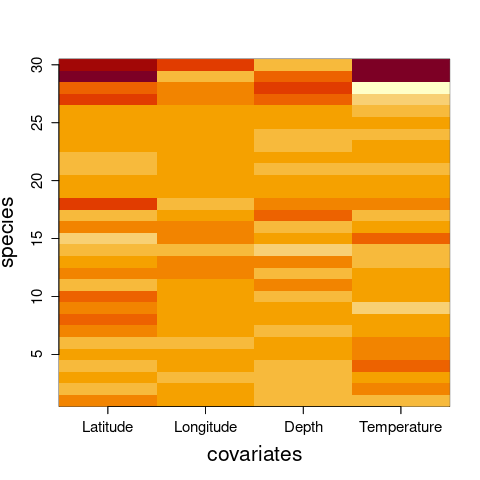
\includegraphics[width=.25\textwidth, trim=0 10 20 10, clip=]{\figbayes/FigUVSQ-BarentsFish-coeffAll-woIntercept-specOrderTRUE} & 
    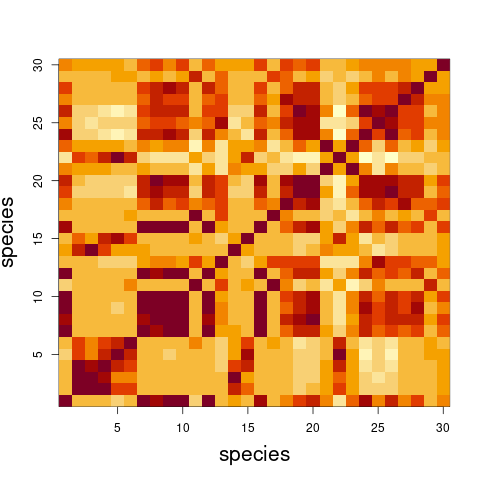
\includegraphics[width=.25\textwidth, trim=0 10 20 10, clip=]{\figbayes/FigUVSQ-BarentsFish-corrPred-specOrderTRUE} & 
    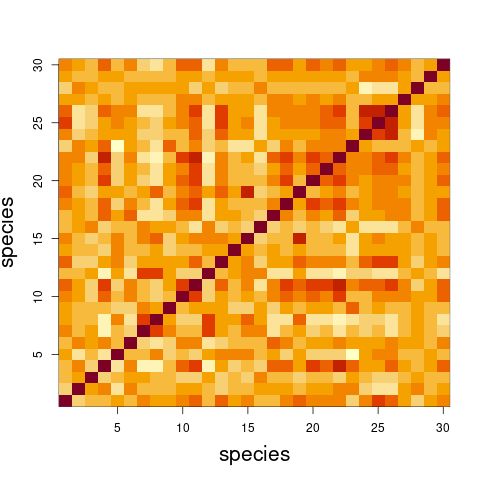
\includegraphics[width=.25\textwidth, trim=0 10 20 10, clip=]{\figbayes/FigUVSQ-BarentsFish-corrAll-specOrderTRUE}
  \end{tabular}
  $$

}

%====================================================================
\frame{\frametitle{Inference} 

  \paragraph{Maximum likelihood inference via EM.} \refer{DLR77}
  $$
  \theta^{(h+1)} 
  = \underset{\text{\normalsize \emphase{M step}}}{\underbrace{\argmax_\theta}} \; \underset{\text{\normalsize \emphase{E step}}}{\underbrace{\Esp_{\theta^{(h)}}}}[\log p_\theta(Y, Z) \mid Y]
  $$
  \begin{itemize}
    \setlength{\itemsep}{.75\baselineskip}
    \item The E step requires some knowledge about $p_\theta(Z \mid Y)$
    \item Which turns out to be intractable for the PLN model.
  \end{itemize}
  
  \bigskip \pause
  \paragraph{Variational EM \refer{WaJ08,BKM17}.} % Replace the E step with an approximation step, i.e.
  \begin{itemize}
    \setlength{\itemsep}{.75\baselineskip}
    \item \pause Choose a class $\Qcal$ of approximate (parametric) distributions and a divergence measure $D[q \| p]$ (e.g. $KL[q \| p]$)
    \item \pause \emphase{VE} step : (approximation)
    $$
    q^{(h+1)} = \argmin_{q \in \emphase{\Qcal}} \emphase{D}\left[q(Z) \| p_{\theta^{(h)}}(Z \mid Y)\right]
    $$
    \item \pause \emphase{M} step : (update)
    $$
    \theta^{(h+1)} = \argmax_\theta \Esp_{\emphase{q^{(h+1)}}}\left[\log p_\theta(Y, Z)\right]
    $$
    \item \pause If $D = KL$, a lower bound of $\log p_\theta(Y)$ ('ELBO') increases at each step 
  \end{itemize}

}

%====================================================================
\frame{\frametitle{VEM for the Poisson log-normal model}

  \paragraph{Approximation class.} Gaussian approximation \refer{CMR18a}
  $$
  q(Z) = \prod_{i=1}^n \Ncal(Z_i; m_i, S_i)
  $$
  \begin{itemize}
  \item Parameter estimate $\widehat{\theta} = (\widehat{\Sigma}, \widehat{\beta})$, 
  \item Approximate conditional distribution $Z_i \mid Y_i \approx \Ncal(\widetilde{m}_i, \widetilde{S}_i)$, 
  \item Lower bound $ELBO(\widehat{\theta}, \widetilde{m}, \widetilde{S})$ (R package \url{PLNmodels})
  \end{itemize}
  
  \bigskip \pause
  \paragraph{Properties.}
  \begin{itemize}
    \setlength{\itemsep}{.75\baselineskip}
    \item Reasonably easy to implement, fast, empirically accurate
    \item But very few theoretical guaranties, does not enjoy the general properties of maximum likelihood (consistency, asymptotic normality, etc.) \\
    \medskip 
    $\to$ No measure of uncertainty (\emphase{no test, no confidence interval}) 
    \item Can we build upon variational inference to achieve 'genuine' statistical inference?
  \end{itemize}
  
}


%====================================================================
%====================================================================
\subsection{Fish species from the Barents sea}
\frame{\frametitle{Back to the Barents sea} 
}
%====================================================================

